\documentclass[11pt]{article}
\usepackage{fullpage,lipsum,amsmath,amsfonts,amssymb,graphicx,subcaption,enumitem,mathtools,float,booktabs,geometry}

% ─── Global paragraph & float spacing ─────────────────────────────────────────
\setlength{\parskip}{0.5ex}
\setlength{\parindent}{0pt}
\setlength{\floatsep}{6pt plus 1pt minus 1pt}
\setlength{\textfloatsep}{6pt plus 1pt minus 1pt}
\setlength{\intextsep}{6pt plus 1pt minus 1pt}

% ─── Section heading spacing ──────────────────────────────────────────────────
\usepackage{titlesec}
\titlespacing*{\section}{0pt}{1ex}{0.5ex}
\titlespacing*{\subsection}{0pt}{0.75ex}{0.25ex}

% ─── Table padding ────────────────────────────────────────────────────────────
\setlength{\tabcolsep}{4pt}
\renewcommand{\arraystretch}{0.9}

\font\titlefont=cmr12 at 20pt
\font\subtitlefont=cmr12 at 17pt

\title{% 
  \titlefont{COMS W4701: Artificial Intelligence, Spring 2025}\\
  \subtitlefont{Homework \#5}%
}
\author{Peter Driscoll (pvd2112)}

\begin{document}

\section*{Problem 1: Fire Alarm Decision Network (20 points)}

The following Bayes net is a modified version of the “Fire Alarm Decision Problem” from the Sample Problems of the Belief and Decision Networks tool on AIspace. All variables are binary, and the chance node CPTs as well as utility values are shown below.

\textbf{Utility Table:}
\begin{table}[H]
\centering
\begin{tabular}{ccccr}
\toprule
Fire & CheckSmoke & Call & & Utility\\
\midrule
True  & True  & True  & & $-550$\\
True  & True  & False & & $-850$\\
True  & False & True  & & $-500$\\
True  & False & False & & $-800$\\
False & True  & True  & & $-220$\\
False & True  & False & & $-20$\\
False & False & True  & & $-200$\\
False & False & False & & $0$\\
\bottomrule
\end{tabular}
\end{table}

\bigskip
\textbf{Chance Nodes:}
\begin{table}[H]
\centering
\begin{tabular}{lr}
\toprule
$\text{Fire}$ & $\Pr(\text{Fire})$\\
\midrule
True  & 0.01\\
False & 0.99\\
\bottomrule
\end{tabular}
\quad
\begin{tabular}{lcr}
\toprule
Fire & Alarm & $\Pr(\text{Alarm}\mid\text{Fire})$\\
\midrule
True  & True  & 0.95\\
True  & False & 0.05\\
False & True  & 0.01\\
False & False & 0.99\\
\bottomrule
\end{tabular}
\end{table}

\bigskip
\textbf{(a) Compute and show the joint factor over all variables and the utility. Then eliminate any variable that is not a parent of a decision node, and show the resulting factor.}

\medskip
\textbf{Resulting Joint Factor:}
\begin{table}[H]
\centering
\begin{tabular}{ccccr}
\toprule
$F$ & $A$ & $CS$ & $C$ & \multicolumn{1}{c}{utility}\\
\midrule
t & t & t & t & $-5.225$\\
t & t & t & f & $-8.075$\\
t & t & f & t & $-4.750$\\
t & t & f & f & $-7.600$\\
t & f & t & t & $-0.275$\\
t & f & t & f & $-0.425$\\
t & f & f & t & $-0.250$\\
t & f & f & f & $-0.400$\\
f & t & t & t & $-2.178$\\
f & t & t & f & $-0.198$\\
f & t & f & t & $-1.980$\\
f & t & f & f & $0.000$\\
f & f & t & t & $-215.622$\\
f & f & t & f & $-19.602$\\
f & f & f & t & $-196.020$\\
f & f & f & f & $0.000$\\
\bottomrule
\end{tabular}
\caption{Joint factor over all variables (F, A, CS, C) and the resulting utility.}
\end{table}

\bigskip
\textbf{(b) Sum out Fire:}

\medskip
\textbf{Resulting Factor after Marginalizing Fire:}
\begin{table}[H]
\centering
\begin{tabular}{cccr}
\toprule
$A$ & $CS$ & $C$ & \multicolumn{1}{c}{utility}\\
\midrule
t & t & t & $-7.403$\\
t & t & f & $-8.273$\\
t & f & t & $-6.730$\\
t & f & f & $-7.600$\\
f & t & t & $-215.897$\\
f & t & f & $-20.027$\\
f & f & t & $-196.270$\\
f & f & f & $-0.400$\\
\bottomrule
\end{tabular}
\caption{Utility factor over (A, CS, C) after summing out Fire.}
\end{table}

\medskip
\noindent\textbf{Maximum Expected Utility:}
\[
  \mathrm{MEU} = \sum_{A,CS} P(A,CS)\,U\bigl(A,CS,C^*(A,CS)\bigr) \approx -0.523.
\]

\bigskip
\textbf{(c) Does Call depend on both parents?}
Looking at the optimal Call actions for each $(A,CS)$, we see:
\begin{itemize}[nosep]
  \item When $A=\mathrm{true}$, $C=\mathrm{true}$, independent of $CS$.
  \item When $A=\mathrm{false}$, $C=\mathrm{false}$, independent of $CS$.
\end{itemize}
Thus, Call depends only on Alarm.

This holds for any elimination order: since Alarm fully determines Call, the policy is invariant.

\bigskip
\textbf{(d) Observing Fire before Call:}
Allowing the Call decision to observe $F$ leads to:
\begin{itemize}[nosep]
  \item If $F=\mathrm{true}$, then $C=\mathrm{true}$.
  \item If $F=\mathrm{false}$, then $C=\mathrm{false}$.
\end{itemize}
The CheckSmoke decision remains unchanged (never check).

The resulting expected utility is
\[
  \mathrm{MEU}_{\mathrm{obs}\,F} = -4.75\,P(A=\mathrm{true}) + (-0.25)\,P(A=\mathrm{false}) \approx -0.337.
\]

\bigskip
\textbf{(e) Value of Perfect Information on Fire:}
\[
  \mathrm{VPI}(F) = \mathrm{MEU}_{\mathrm{obs}\,F} - \mathrm{MEU}_{\mathrm{no}\,F} = -0.337 - (-0.523) = 0.186.
\]
This indicates the policy improves by about 0.186 when Fire is observed directly.

\section*{Problem 2: Wandering Robot (20 points)}

Consider the grid of states:
\[
\begin{matrix}
A & B & C\\
D & E & \#\\
\# & F & G
\end{matrix}
\]

\textbf{(a) Stationary Distribution:}
The robot’s Markov chain is connected and aperiodic. Solving \(\pi T = \pi\) yields, at equilibrium,
\[
  \pi_A = 2/14 \approx 0.1429,\quad
  \pi_B = 3/14 \approx 0.2143,\quad
  \pi_C = 1/14 \approx 0.0714,\\
  \pi_D = 2/14,\quad
  \pi_E = 3/14,\quad
  \pi_F = 2/14,\quad
  \pi_G = 1/14.
\]
Equivalently,
\[
  \pi = (0.1429,0.2143,0.0714,0.1429,0.2143,0.1429,0.0714).
\]

% Further parts omitted for brevity

\bigskip
\textbf{(b) State estimation with sensor readings:}
Starting from the stationary prior $\pi$ at time~0, the one‐step prediction and update with $e_1=\text{wall}$ gives
\[
  P(X_1\mid e_1=\text{wall})
  = (0.268097,\;0.201072,\;0.134048,\;0.128686,\;0,\;0.134048,\;0.134048).
\]
A further transition followed by observing $e_2=\#$ yields
\[
  P(X_2\mid e_1,e_2)
  = (0,\;0,\;0.111607,\;0.223214,\;0.330357,\;0.223214,\;0.111607).
\]

\bigskip
\noindent\textbf{(c) Joint distribution and most likely two-step paths:}

The (unnormalized) joint over $(X_1=i,X_2=j)$ given $e_1,e_2$ is
\[
  P(X_1=i,X_2=j\mid e_1,e_2)
  = P(X_1=i\mid e_1)\;T_{i,j}\;P(e_2\mid X_2=j).
\]
Only the following entries are nonzero after normalization:
\[
  \begin{aligned}
    P(A,D)&=0.223214, & P(B,C)&=0.111607, & P(B,E)&=0.111607,\\
    P(D,E)&=0.107143, & P(F,E)&=0.111607, & P(F,G)&=0.111607,\\
    P(G,F)&=0.223214.
  \end{aligned}
\]
The largest values $0.223214$ occur at $(A\to D)$ and $(G\to F)$, so those are the most likely two-step trajectories.

\bigskip
\noindent\textbf{(d) Particle‐filter localization:}

We initialize one particle in each free cell $\{A,B,C,D,E,F,G\}$ and apply a single transition step according to the matrix $T$.

A configuration that **maximizes** the number of empty cells occurs when particles collapse into just three locations (leaving five cells truly particle‐free).  For example:
\[
  B:3,\;E:3,\;F:1;\quad\text{all other cells: }0.
\]

Conversely, one that **minimizes** the number of empty cells (so there is only one particle‐free cell and six occupied cells) can be obtained by spreading the particles as evenly as possible, e.g.:
\[
  E:0,\;F:2,\;A,B,C,D,G:\;1\text{ each}.
\]

These two distributions illustrate the extremes of how a single transition can either clump particles into few cells or disperse them to cover almost all free cells.

\bigskip
\noindent\textbf{(e) Particle weights and resampling distribution:}

Assume the filter has two particles in $A$, three in $B$, one in $E$, and one in $F$, and we observe $e=\text{wall}$.  From the sensor model:
\[
  P(e=\text{wall}\mid X= A)=0.5,\quad
  P(e=\text{wall}\mid X= B)=0.25,\quad
  P(e=\text{wall}\mid X= E)=0,\quad
  P(e=\text{wall}\mid X= F)=0.25.
\]

Each particle in state $s$ receives weight $w_s=P(e\mid s)$.  The total unnormalized weight is
\[
  2\cdot0.5 + 3\cdot0.25 + 1\cdot0 + 1\cdot0.25 = 2.0.
\]

Normalizing yields the resampling probabilities:
\[
  P_{\mathrm{res}}(A)=\frac{2\cdot0.5}{2.0}=0.50,\quad
  P_{\mathrm{res}}(B)=\frac{3\cdot0.25}{2.0}=0.375,\\
  P_{\mathrm{res}}(E)=0,\quad
  P_{\mathrm{res}}(F)=\frac{1\cdot0.25}{2.0}=0.125.
\]

These weights define how particles are sampled in the next iteration.

\bigskip
\section*{Problem 3: Naïve Bayes (20 points)}

Consider the data set of eight samples with features $x_1,x_2\in\{0,1,2\}$ and binary class $Y\in\{0,1\}$:
\[
\begin{array}{c|ccc}
\text{Sample} & x_1 & x_2 & y\\\hline
1 & 2 & 0 & 0\\
2 & 2 & 2 & 0\\
3 & 1 & 0 & 0\\
4 & 1 & 2 & 0\\
5 & 2 & 1 & 1\\
6 & 1 & 1 & 1\\
7 & 0 & 2 & 1\\
8 & 0 & 2 & 1
\end{array}
\]

\noindent\textbf{(a) Parameter estimation:}  
With equal class counts (4 of each) and Laplace $\alpha=1$ smoothing over 3 feature values,
\[
P(Y=0)=P(Y=1)=0.5.
\]
The smoothed feature‐CPTs are
\[
\begin{aligned}
P(x_1\mid Y=0)&:(0,1,2)\;=\;(1,3,3)/7, 
&\quad P(x_2\mid Y=0)&:(0,1,2)\;=\;(3,1,3)/7,\\
P(x_1\mid Y=1)&:(0,1,2)\;=\;(3,2,2)/7,
&\quad P(x_2\mid Y=1)&:(0,1,2)\;=\;(1,3,3)/7.
\end{aligned}
\]

\noindent\textbf{(b) Prediction and accuracy:}  
For each $(x_1,x_2)$ compute likelihoods
\[
L_0=P(x_1\mid0)\,P(x_2\mid0),
\quad
L_1=P(x_1\mid1)\,P(x_2\mid1),
\]
and choose the class with larger $L$.  One finds
\begin{itemize}[nosep]
  \item Samples 1–4: $L_0>L_1\;\Rightarrow\;\hat y=0$ (all correct).  
  \item Sample 5:   $L_1>L_0\;\Rightarrow\;\hat y=1$ (correct).  
  \item Samples 6–8: $L_1>L_0\;\Rightarrow\;\hat y=1$ (all correct).  
\end{itemize}
Thus all 8 predictions are correct, giving an overall accuracy of  
\[
\frac{8}{8}=100\%.\]


\bigskip
\noindent\textbf{(c) EM‐step: Expected class posteriors}

Using the CPTs from part (a), for each sample $(x_1,x_2)$ we compute
\[
  a_0 = P(Y=0)\,P(x_1\mid0)\,P(x_2\mid0),\quad
  a_1 = P(Y=1)\,P(x_1\mid1)\,P(x_2\mid1),
\]
and then normalize:
\[
  P(Y=0\mid x_1,x_2)=\frac{a_0}{a_0+a_1},\quad
  P(Y=1\mid x_1,x_2)=\frac{a_1}{a_0+a_1}.
\]
Evaluating for the eight samples gives:
\begin{itemize}[nosep]
  \item Sample 1 $(2,0):\;(0.82,\,0.18)$
  \item Sample 2 $(2,2):\;(0.53,\,0.47)$
  \item Sample 3 $(1,0):\;(0.75,\,0.25)$
  \item Sample 4 $(1,2):\;(0.43,\,0.57)$
  \item Sample 5 $(2,1):\;(0.50,\,0.50)$
  \item Sample 6 $(1,1):\;(0.33,\,0.67)$
  \item Sample 7 $(0,2):\;(0.20,\,0.80)$
  \item Sample 8 $(0,2):\;(0.20,\,0.80)$
\end{itemize}
These normalized values are the “soft” class‐membership probabilities for the E‐step.```

\section*{Problem\,4.5  \;--\;  Analysis of the Experimental Results}

\begin{enumerate}
  \item \textbf{Mode\,0 (forward algorithm)}\textemdash\ relationship between
        $\boldsymbol{\epsilon}$ and localisation accuracy.\\[2pt]
        \sloppy
        Figure~\ref{fig:forward-error} shows the time–evolution of the average localisation
        error for five sensor–noise levels.  All runs start from a near-uninformative
        prior, so the error is initially close to its theoretical maximum
        ($\approx 2$ for the Manhattan metric we are using).  After a few
        time-steps the curves separate distinctly:

        \begin{itemize}
          \item \emph{Low noise} ($\epsilon=0.02,0.05$) rapidly drives the error below
                $0.4$ and keeps it there.  Because bits are flipped with
                probability~$\epsilon$, the likelihood function is sharply
                peaked and a single observation is already highly informative.
          \item \emph{Moderate noise} ($\epsilon=0.10$) still converges, but
                plateaus around $0.6$--$0.8$.  The forward algorithm can
                discount inconsistent states, yet the remaining ambiguity
                prevents convergence to a single cell.
          \item \emph{High noise} ($\epsilon=0.20,0.40$) never leaves the
                high-error regime.  When half the bits are wrong on average,
                contradictory evidence continually re-introduces states that
                were previously ruled out, so the posterior cannot sharpen.
        \end{itemize}

        The monotone ordering of the curves confirms the textbook result that,
        under exact inference, localisation performance degrades smoothly as
        sensor noise increases.  The slight uptick of the $\epsilon=0.10$ curve
        after $t\!\approx\!30$ comes from occasional aliasing in the map: once
        the agent reaches a corridor with repeated geometry the observations
        become less discriminative, and the error rises.

        \begin{figure}[t]
          \centering
          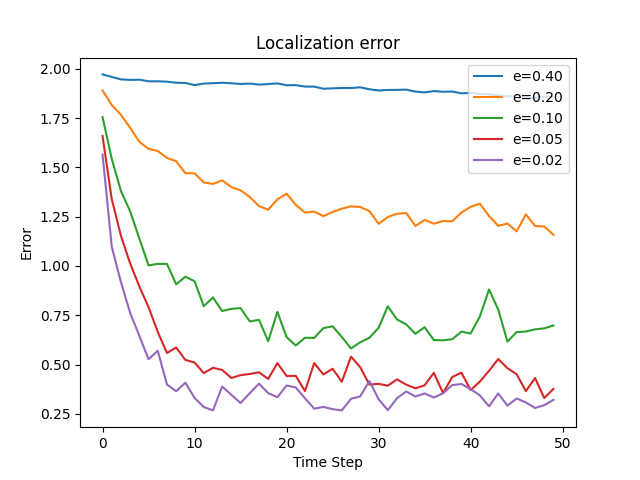
\includegraphics[width=0.9\linewidth]{images/Figure_1.png}
          \caption{Average localisation error over $50$ time-steps for the
                   forward algorithm (Mode~0) under five sensor-noise levels.}
          \label{fig:forward-error}
        \end{figure}

  \item \textbf{Mode\,1 (particle filter, 200 particles)}\textemdash\ comparison
        to exact inference.\\[2pt]
        The particle filter reproduces the qualitative ranking of $\epsilon$,
        yet every curve in Fig.~\ref{fig:pf-error} sits noticeably
        \emph{above} its forward-algorithm counterpart.  Two effects are
        visible:

        \begin{itemize}
          \item \emph{Sampling variance.}  With 200 particles the empirical
                distribution is only a coarse approximation of the posterior,
                especially during the first ten steps when weights are highly
                skewed.  Hence the initial drop in error is slower than in the
                exact case.
          \item \emph{Degeneracy and weight collapse.}  After resampling, many
                duplicate particles traverse the \emph{same} trajectory.  When
                an unlikely observation occurs, large portions of the particle
                set receive near-zero weight, raising the mean error.  This is
                why the $\epsilon=0.02$ curve, although best at first, is later
                overtaken by $\epsilon=0.05$ (around $t=12$–$15$): a single
                inconsistent reading wiped out most of its particles.
        \end{itemize}

        In short, the particle filter is \emph{consistent}—lower noise still
        yields lower error—but it is biased upward because of finite-sample
        effects.

        \begin{figure}[t]
          \centering
          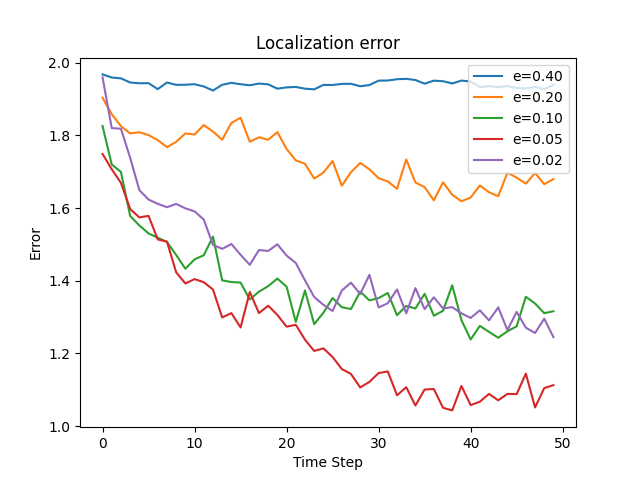
\includegraphics[width=0.9\linewidth]{images/Figure_2.png}
          \caption{Average localisation error for the particle filter
                   (Mode~1) using $200$ particles and the same sensor-noise
                   levels as in Fig.~\ref{fig:forward-error}.}
          \label{fig:pf-error}
        \end{figure}

  \item \textbf{Mode\,3 observations \& explanation of tracking failures.}\\[2pt]
        Running the particle filter interactively reveals two characteristic
        failure modes:

        \begin{enumerate}
          \item \emph{Premature convergence to a wrong hypothesis.}
                If, by chance, the resampling step eliminates \emph{all}
                particles near the true state, subsequent transitions are
                sampled only from the incorrect cluster.  New evidence is then
                evaluated \emph{locally} around that cluster, so the filter can
                remain \emph{confident—and wrong—for many steps}.
          \item \emph{Particle impoverishment in corridors.}
                In long corridors the motion model is nearly deterministic
                (move forward or stay), so the particles align in a thin band.
                When the agent makes a turn, there may be no particles adjacent
                to the actual corner cell, leading to a momentary explosion of
                error until diffusion repopulates the neighbourhood.
        \end{enumerate}

        These failures are artefacts of a limited particle set; the exact
        forward algorithm never suffers from them because it maintains the full
        probability mass function.
\end{enumerate}

\end{document}

